\section{The Turret}\label{turret}
The turret is purpose-built using LEGO bricks following a custom design made by the project group. The turret consists of three main parts: the cannon, the sensory system and the rotation system. A total of three motors are mounted on the turret to aid the cannon and the rotation system, using the three motors selected in \cref{sec:actuators}. The turret with sensors and motors mounted can be seen in \cref{turret1}. The requirement to keep the turret autonomous, was interpreted as the turret needing to be \enquote{one unit}, meaning that all of the turrets components had to be in direct contact with the rest. This was chosen in order to keep true to the idea of the tower defense game, by making the placement of a tower a simple process.

\imgscale{figures/turret.png}{The turret with infrared sensors mounted}{turret1}{0.19}

On \cref{fig:turret2,fig:turret3} a cross section of the turret can be seen, and the description will refer to the figures. The turret uses LEGO bricks as projectiles (C). These projectiles are fired by releasing a piston bolt (B) from a retracted position, seen on \cref{fig:turret3}. The bolt, when released, is pulled into the barrel (D) by stretched elastic bands which contract and push the bolt into the loaded projectile (G), propelling it out of the barrel. The elastic bands are stretched using motor driven rotating rods (A), which in a circular pattern pull the bolt back to the apex of the stretch, and then sliding off the bolt, releasing it and allowing the elastic bands to contract. This allows for automatic fire of projectiles by continuously rotating the rods, however, it also makes priming the cannon in a cocked position difficult. The turret is loaded when the bolt is retracted as this allows a LEGO brick to drop down into the chamber just prior to the release of the bolt, as can be seen in \cref{fig:turret3}. The turret can hold a magazine with a capacity of 10 projectiles.

\begin{figure}[H]
\begin{center}
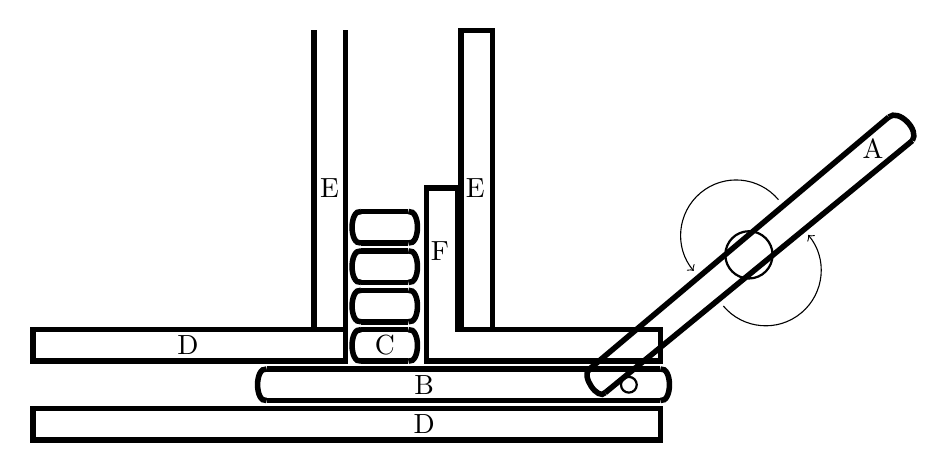
\begin{tikzpicture}


    
    \draw [line width=2](0,-0.2) -- (8,-0.2) -- (8,0.2) -- (0.03,0.2) -- (0.03,-0.2);
    \draw [line width=2](3.6,5) -- (3.6,1.2) -- (4,1.2) -- (4,5);
    \draw [line width=2](0,0.8) -- (4,0.8) -- (4,1.2) -- (0.03,1.2) -- (0.03,0.8);
    \draw [line width=2](5.0,0.8) -- (8,0.8) -- (8,1.2) -- (5.43,1.2) -- (5.43,3) -- (5.03,3) -- (5.03,0.8);
    \draw [line width=2](5.87,1.2) -- (5.87,5) -- (5.47,5) -- (5.47,1.2);
    %\draw [-triangle 90,fill=black](1.7,3) -- (1.7,2);
    %\draw [triangle 90-triangle 90,fill=green, color=blue](2,1.5) -- (4,1.5);
    %\node at (5,3.5) {arm/cpu};
    
    \coordinate (A) at (4.2,0.8);
    \coordinate (B) at (4.8,0.8);
    \coordinate (C) at (4.2,1.2);
    \coordinate (D) at (4.8,1.2);
    
    \draw[line width=2pt] (A) to[out=190,in=-190] (C);
    \draw[line width=2pt] (B) to[out=-10,in=10] (D);
    \draw[line width=2pt] (A) -- (B);
    \draw[line width=2pt] (C) -- (D);
    
    \coordinate (E) at (4.2,1.3);
    \coordinate (F) at (4.8,1.3);
    \coordinate (G) at (4.2,1.7);
    \coordinate (H) at (4.8,1.7);
    
    \draw[line width=2pt] (E) to[out=190,in=-190] (G);
    \draw[line width=2pt] (F) to[out=-10,in=10] (H);
    \draw[line width=2pt] (E) -- (F);
    \draw[line width=2pt] (G) -- (H);
    
    \coordinate (M) at (4.2,1.8);
    \coordinate (N) at (4.8,1.8);
    \coordinate (O) at (4.2,2.2);
    \coordinate (P) at (4.8,2.2);
    
    \draw[line width=2pt] (M) to[out=190,in=-190] (O);
    \draw[line width=2pt] (N) to[out=-10,in=10] (P);
    \draw[line width=2pt] (M) -- (N);
    \draw[line width=2pt] (O) -- (P);
    
    %rotating rod
    \coordinate (I) at (7.1,0.7);
    \coordinate (J) at (7.3,0.4);
    \coordinate (K) at (10.9,3.9);
    \coordinate (L) at (11.2,3.6);
    
    \draw[line width=2pt] (I) to[out=215,in=230] (J);
    \draw[line width=2pt] (K) to[out=40,in=55] (L);
    \draw[line width=2pt] (I) -- (K);
    \draw[line width=2pt] (J) -- (L);

    \draw[line width=0.8pt] (9.125,2.15) circle (3mm);
    \draw [->] (9.5,2.85) arc (40:220:20pt);
    \draw [->] (8.8,1.5) arc (220:400:20pt);
    
    \coordinate (Q) at (3,0.3);
    \coordinate (R) at (8,0.3);
    \coordinate (S) at (3,0.7);
    \coordinate (T) at (8,0.7);
    
    \draw[line width=2pt] (Q) to[out=190,in=-190] (S);
    \draw[line width=2pt] (R) to[out=-10,in=10] (T);
    \draw[line width=2pt] (Q) -- (R);
    \draw[line width=2pt] (S) -- (T);
    
    \draw[line width=0.8pt] (7.6,0.5) circle (1mm);    
    
    \coordinate (U) at (4.2,2.3);
    \coordinate (X) at (4.8,2.3);
    \coordinate (Y) at (4.2,2.7);
    \coordinate (Z) at (4.8,2.7);
    
    \draw[line width=2pt] (U) to[out=190,in=-190] (Y);
    \draw[line width=2pt] (X) to[out=-10,in=10] (Z);
    \draw[line width=2pt] (U) -- (X);
    \draw[line width=2pt] (Y) -- (Z);
    
    
    \node at (10.7,3.5) {A};
    \node at (5,0.5) {B};
    \node at (4.5,1) {C};
    \node at (5,0) {D};
    \node at (2,1) {D};
    \node at (5.65,3) {E};
    \node at (3.8,3) {E};
    \node at (5.2,2.2) {F};
    
\end{tikzpicture}
\end{center}
\caption{Turret before loading/after shooting}
\label{fig:turret2}
\end{figure}


\begin{figure}[H]
\begin{center}
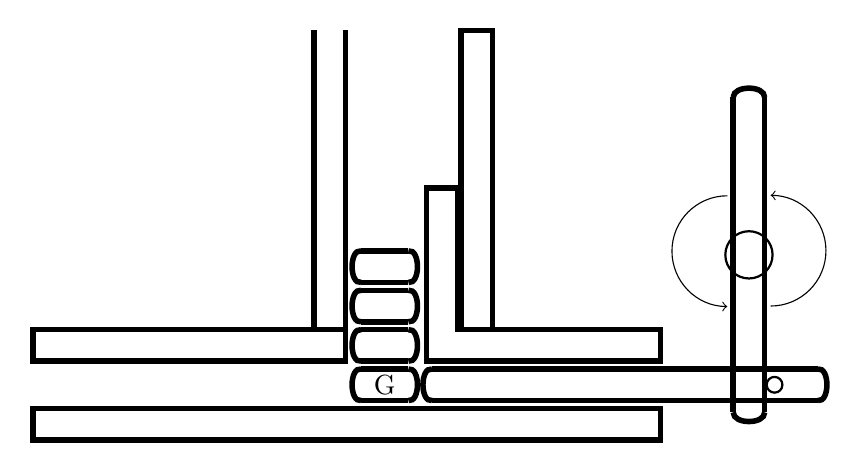
\begin{tikzpicture}

    \draw [line width=2](0,-0.2) -- (8,-0.2) -- (8,0.2) -- (0.03,0.2) -- (0.03,-0.2);
    \draw [line width=2](3.6,5) -- (3.6,1.2) -- (4,1.2) -- (4,5);
    \draw [line width=2](0,0.8) -- (4,0.8) -- (4,1.2) -- (0.03,1.2) -- (0.03,0.8);
    \draw [line width=2](5.0,0.8) -- (8,0.8) -- (8,1.2) -- (5.43,1.2) -- (5.43,3) -- (5.03,3) -- (5.03,0.8);
    \draw [line width=2](5.87,1.2) -- (5.87,5) -- (5.47,5) -- (5.47,1.2);
    %\draw [-triangle 90,fill=black](1.7,3) -- (1.7,2);
    %\draw [triangle 90-triangle 90,fill=green, color=blue](2,1.5) -- (4,1.5);
    %\node at (5,3.5) {arm/cpu};
    
    %shots
    \coordinate (A) at (4.2,0.8);
    \coordinate (B) at (4.8,0.8);
    \coordinate (C) at (4.2,1.2);
    \coordinate (D) at (4.8,1.2);
    
    \draw[line width=2pt] (A) to[out=190,in=-190] (C);
    \draw[line width=2pt] (B) to[out=-10,in=10] (D);
    \draw[line width=2pt] (A) -- (B);
    \draw[line width=2pt] (C) -- (D);
    
    \coordinate (E) at (4.2,1.3);
    \coordinate (F) at (4.8,1.3);
    \coordinate (G) at (4.2,1.7);
    \coordinate (H) at (4.8,1.7);
    
    \draw[line width=2pt] (E) to[out=190,in=-190] (G);
    \draw[line width=2pt] (F) to[out=-10,in=10] (H);
    \draw[line width=2pt] (E) -- (F);
    \draw[line width=2pt] (G) -- (H);
    
    \coordinate (M) at (4.2,1.8);
    \coordinate (N) at (4.8,1.8);
    \coordinate (O) at (4.2,2.2);
    \coordinate (P) at (4.8,2.2);
    
    \draw[line width=2pt] (M) to[out=190,in=-190] (O);
    \draw[line width=2pt] (N) to[out=-10,in=10] (P);
    \draw[line width=2pt] (M) -- (N);
    \draw[line width=2pt] (O) -- (P);

    \coordinate (U) at (4.2,0.3);
    \coordinate (X) at (4.8,0.3);
    \coordinate (Y) at (4.2,0.7);
    \coordinate (Z) at (4.8,0.7);
    
    \draw[line width=2pt] (U) to[out=190,in=-190] (Y);
    \draw[line width=2pt] (X) to[out=-10,in=10] (Z);
    \draw[line width=2pt] (U) -- (X);
    \draw[line width=2pt] (Y) -- (Z);
    
    %Rotating rod
    \coordinate (I) at (9.325,4.15);
    \coordinate (J) at (8.925,4.15);
    \coordinate (K) at (9.325,0.15);
    \coordinate (L) at (8.925,0.15);
    
    \draw[line width=2pt] (I) to[out=90,in=90] (J);
    \draw[line width=2pt] (K) to[out=270,in=270] (L);
    \draw[line width=2pt] (I) -- (K);
    \draw[line width=2pt] (J) -- (L);

    \draw[line width=0.8pt] (9.125,2.15) circle (3mm);
    \draw [->] (8.85,2.9) arc (90:270:20pt);
    \draw [->] (9.4,1.5) arc (270:450:20pt);
    
    %piston
    \coordinate (Q) at (5.1,0.3);
    \coordinate (R) at (10,0.3);
    \coordinate (S) at (5.1,0.7);
    \coordinate (T) at (10,0.7);
    
    \draw[line width=2pt] (Q) to[out=190,in=-190] (S);
    \draw[line width=2pt] (R) to[out=-10,in=10] (T);
    \draw[line width=2pt] (Q) -- (R);
    \draw[line width=2pt] (S) -- (T);
    
    \draw[line width=0.8pt] (9.45,0.5) circle (1mm);    
    
    \node at (4.5,0.5) {G};
    
\end{tikzpicture}
\end{center}
\caption{Turret while loaded}
\label{fig:turret3}
\end{figure}




